\documentclass{beamer}

\usepackage[utf8]{inputenc}
\usepackage[T1]{fontenc}
\usepackage[english]{babel}
\usepackage{graphicx}
\usepackage{animate}

\usepackage{amsthm}
\usepackage{amssymb}
\usepackage{amsmath}

\graphicspath{{./slike/}}

\usetheme{Berlin}
\usecolortheme{default}

\title{Cellular automata}
\author{Tomaž Jonatan Leonardis, Jakob Schrader, Patrik Žnidaršič}
\date{November 6}

\begin{document}

\begin{frame}
  \maketitle
\end{frame}

% TODO Remove this before sending to professor!
\begin{frame}{Title of example frame}
  \begin{block}{Title of block}
	Text in first block
  \end{block}
  \begin{exampleblock}{}
	Text in example block
  \end{exampleblock}
  \begin{theorem}
	This is an important theorem.
  \end{theorem}
\end{frame}

\section{2D variations}

\begin{frame}{2 dimensional variations}
	\begin{block}{}
		We can vary the rules and space of two-dimensional cellular automata in
		multiple ways:
		\begin{itemize}
			\only<+->{\item different tilings (triangles, hexagons, penrose \dots),}
			\only<+->{\item more states (usually denoted with colors),}	%	already said?
			\only<+->{\item accounting for different positions,}
			\only<+(-1)->{\item \dots.}
		\end{itemize}
	\end{block}
	\only<1>{\begin{center}
\includegraphics[width=.4\textwidth]{penrose_tiling.png}\end{center}}
\end{frame}

\section{Life}

\begin{frame}{The Game of Life}
	\begin{block}{Conway's Game of Life}<+->
		In 1970 John Horton Conway devised \textit{The Game of Life}, which is
		played in a 2-dimensional grid with two possible states for each cell, with
		the rules:
		\begin{enumerate}
			\item<+-> Every dead cell with exactly \( 3 \) live neighbours becomes alive,
			otherwise it stays dead.
			\item<+-> Every live cell with exactly \( 2 \) or \( 3 \) live neighbours
			stays alive, otherwise it dies.
		\end{enumerate}
	\end{block}

	\begin{block}{Rule string notation}<+->
		B3/S23 (B - born, S - survives)	%	TODO reword
	\end{block}
\end{frame}

\begin{frame}{Common constructs in Life}
	\only<+>{
		\begin{block}{Still lifes}
			Retain their shape through generations.
		\end{block}
		\begin{center}
			%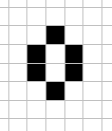
\includegraphics[width=0.2\textwidth]{still_beehive.png}
			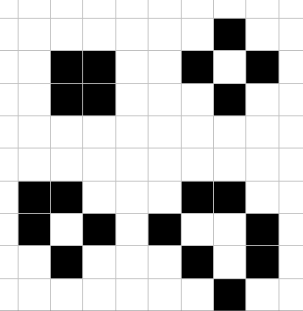
\includegraphics[width=0.4\textwidth]{stills.png}
		\end{center}
	}

	\only<2-3>{
		\begin{block}{Oscillators}
			Loop through a finite number of states and stays in the same location.
		\end{block}
		\begin{center}
			\only<2>{
				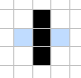
\includegraphics[width=0.3\textwidth]{oscilator_bar.png}
				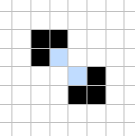
\includegraphics[width=0.3\textwidth]{oscilator_blocks.png}
			}

			\only<3>{
				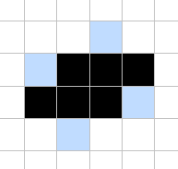
\includegraphics[width=0.3\textwidth]{oscilator_toad3.png}
				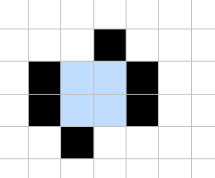
\includegraphics[width=0.3\textwidth]{oscilator_toad2.png}
			}
		\end{center}
	}

	\only<+(2)->{
		\begin{block}{Spaceships}
			Loop through a finite number of states and moves across the field. The most
			notable one is the glider.
		\end{block}

		\begin{center}
			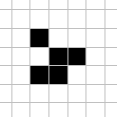
\includegraphics[width=0.17\textwidth]{glider_1.png}
			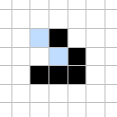
\includegraphics[width=0.17\textwidth]{glider_2.png}
			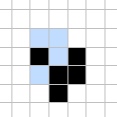
\includegraphics[width=0.17\textwidth]{glider_3.png}
			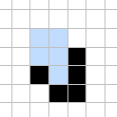
\includegraphics[width=0.17\textwidth]{glider_4.png}
			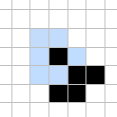
\includegraphics[width=0.17\textwidth]{glider_5.png}
		\end{center}

		\begin{center}
			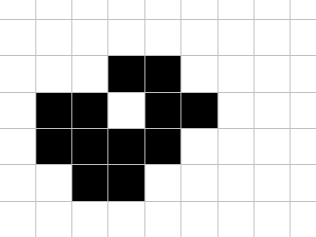
\includegraphics[width=0.17\textwidth]{spaceship_1.png}
			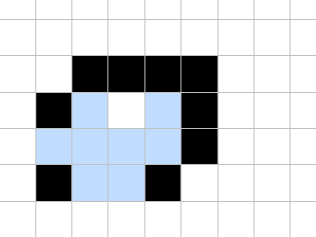
\includegraphics[width=0.17\textwidth]{spaceship_2.png}
			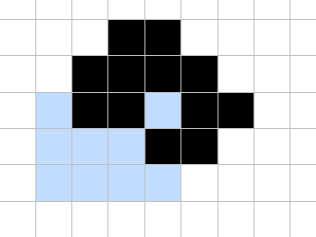
\includegraphics[width=0.17\textwidth]{spaceship_3.png}
			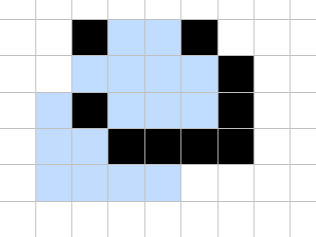
\includegraphics[width=0.17\textwidth]{spaceship_4.png}
			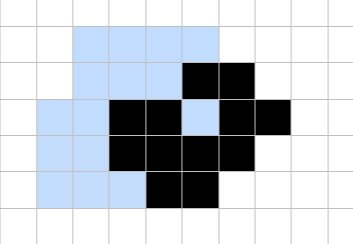
\includegraphics[width=0.17\textwidth]{spaceship_5.png}
		\end{center}
	}

\end{frame}

\section{Introduction of cellular automata}

\begin{frame}{Introduction and history }
 \begin{columns}
     \begin{column}{0.6\textwidth}
          \begin{block}{}

    \begin{itemize}
    \item
    \textbf{Computational model} introduced by John Von Neumann and Stanislaw Ulam in the 1940s
    \item
    It consists of a \textbf{grid of cells}, each in one of a finite number of \textbf{states} that change in \textbf{discrete time} steps according to a \textbf{fixed rule} based on cell's \textbf{neighbourhood}
        \item \textbf{Famous examples:}  Wolfram's elementary cellular automata (1980s), Conway's Game of Life (1970s)...
    \end{itemize}
  \end{block}
     \end{column}
    \column{0.4\textwidth}
        \centering
        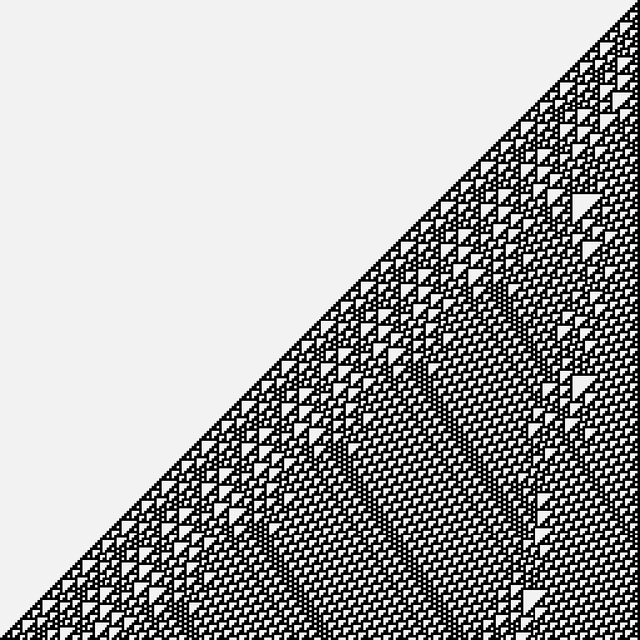
\includegraphics[height=0.4\textheight]{Sample_run_of_Rule_110.png}
        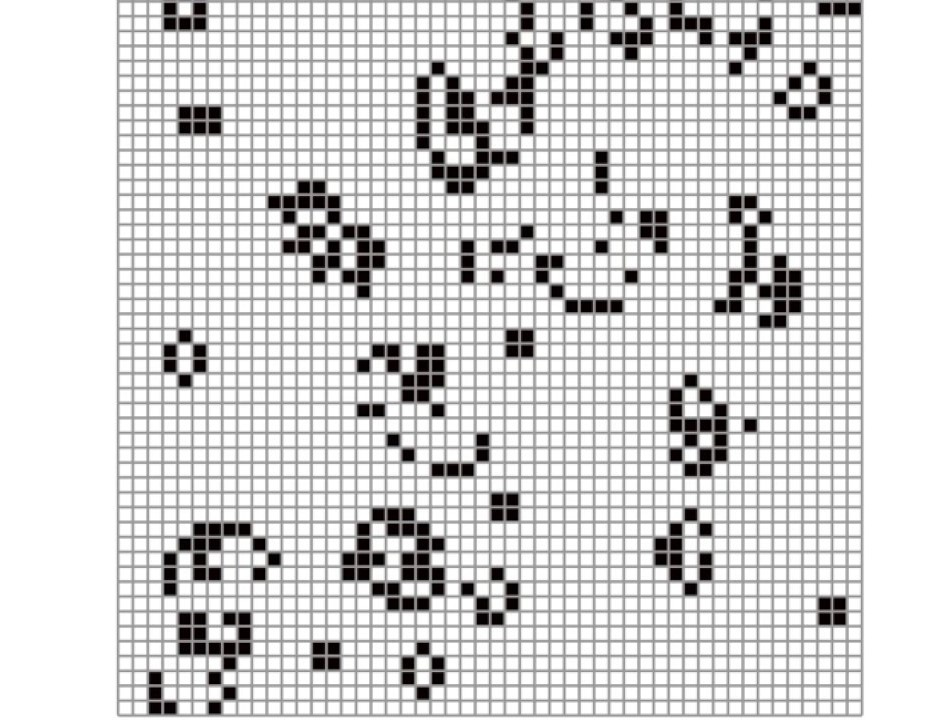
\includegraphics[height=0.4\textheight]{conwaygame.jpg}
 \end{columns}
\end{frame}


\begin{frame}{Core Idea}

\begin{columns}
    \begin{column}{0.8\textwidth}
                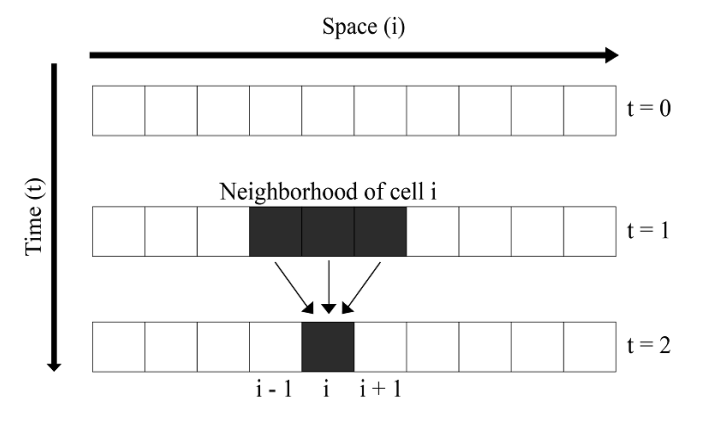
\includegraphics[width = 1.0\textwidth]{slike/intro.png}

    \end{column}
    \begin{column}{0.5\textwidth}
                    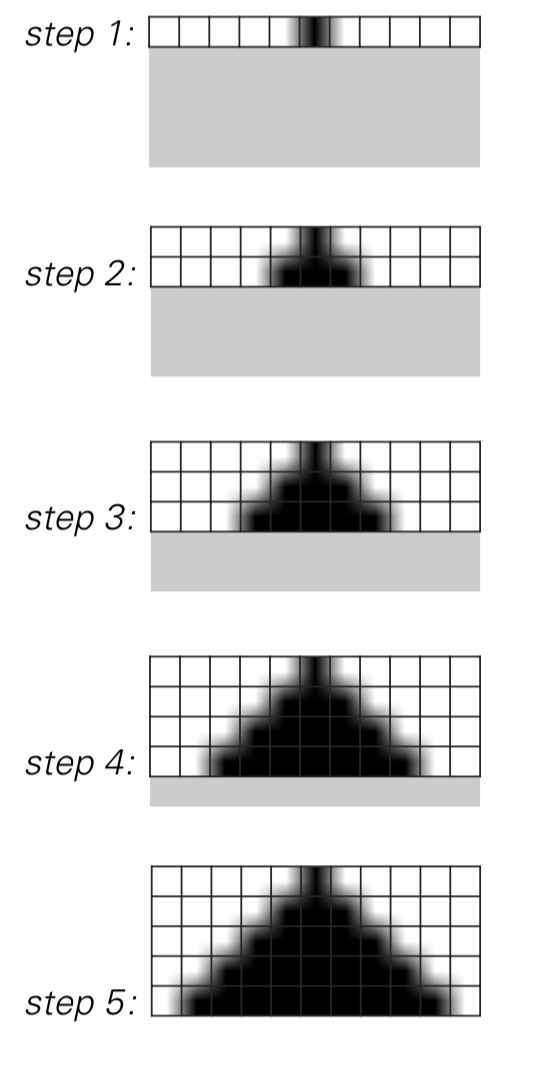
\includegraphics[width = 0.6\textwidth]{timeprogression.jpg}

    \end{column}
\end{columns}

\end{frame}

\begin{frame}{Motivating example (Rule 90)}
  \begin{exampleblock}{}
      \centering
    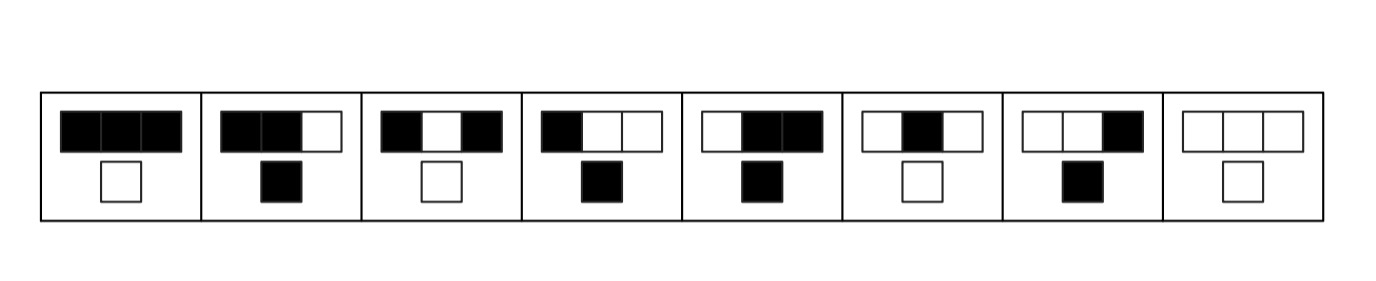
\includegraphics[width = 0.8\textwidth]{Rule90.jpeg}
  \end{exampleblock}
  \begin{block}{Cellular State Space}
  Two states: black - 1 (live), white  - 0 (dead)
  \end{block}
  \begin{block}{Update Rule}
    At each time step: XOR of two neighbouring values
  \end{block}
\end{frame}

\begin{frame}{Motivating example (Rule 90)}
\begin{columns}
    \begin{column}{0.5\textwidth}
                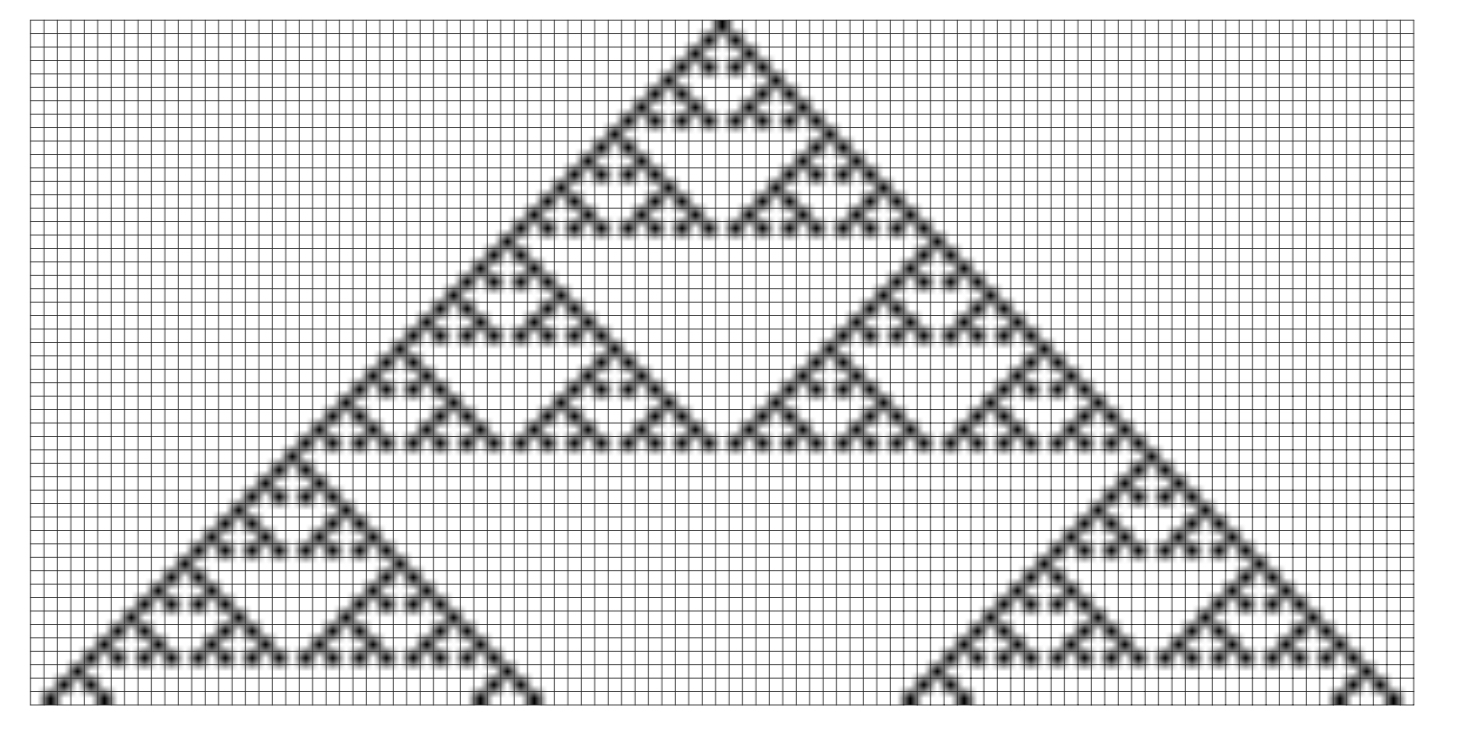
\includegraphics[width = 1.0\textwidth]{slike/rule90evolution.jpeg}
                Sierpinski triangle (from a single live cell)
    \end{column}
    \begin{column}{0.5\textwidth}
                    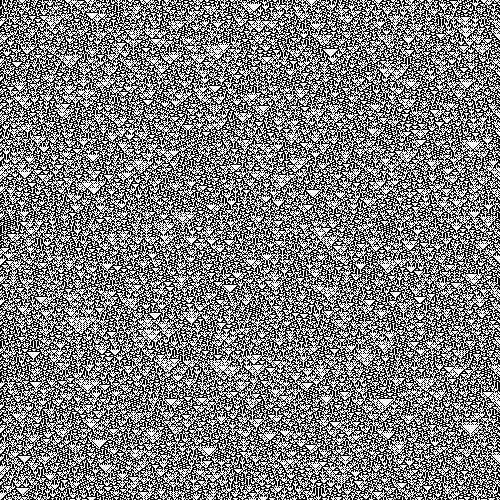
\includegraphics[width = 0.9\textwidth]{randomrule90.png}
                    Time space diagram (random initial conditions)
    \end{column}
\end{columns}

\end{frame}

\begin{frame}{Notations and definition}
	  \begin{itemize}
	  \item \textbf{Discrete cellular state space} $\mathcal{L}$: $n$-dimensional lattice of cells of possibly different shapes (usually homogenous)
	  \item \textbf{Local value space} $\Sigma$: Each cell is in exactly \textbf{one state} $$\sigma_{\vec{i}\in \mathcal{L}}(t) \in \Sigma\equiv \{0,1,2,\dots,k-1 \}$$ The number of possible states is  $k =|\Sigma|$.
   \item \textbf{Boundary conditions} (when the simulation is run on finite sets)
	  \item \textbf{Dynamical rule} $\phi: \Sigma^n \to \Sigma$, where $n$ specifies the number of cells of the neighbourhood $\mathcal{N}\{\vec{i}\}$ about cell $\vec{i}$. Transition rule is written as
        $$\sigma_{\vec{i}}(t+1) = \phi(\sigma_{\vec{j}}(t)\in \mathcal{N}\{\vec{i}\})$$
	  \end{itemize}



\end{frame}


\begin{frame}{One-dimensional example}

  \begin{columns}
	\begin{column}{0.5\textwidth}
	  \begin{itemize}
	  \item One-dimensional lattice
	  \item $\Sigma =\{0,1\}, k = 2$
	  \item No boundary conditions
        \item Neighbourhood of a cell having radius $r=1$ (to the left and right
					of the cell)
        \item Dynamical rule represented with a diagram for $k^{2r+1} = 8$ neighbourhood states.
        \item $k^{k^{2r+1}}=2^8= 256$ possible different rules
	  \end{itemize}

	\end{column}
	\begin{column}{0.7\textwidth}
 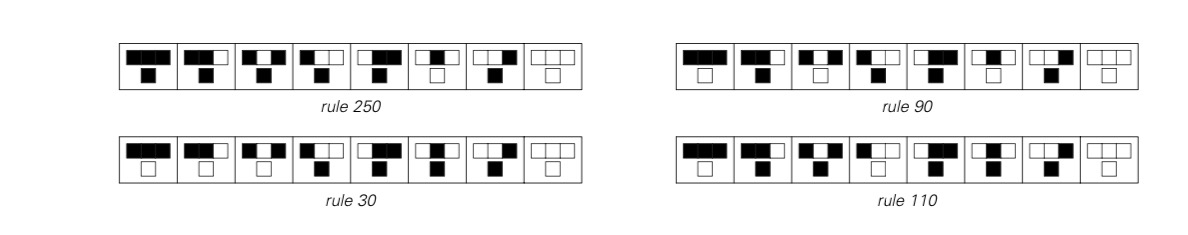
\includegraphics[height=0.18\textheight]{slike/rules.jpeg}
        \centering

        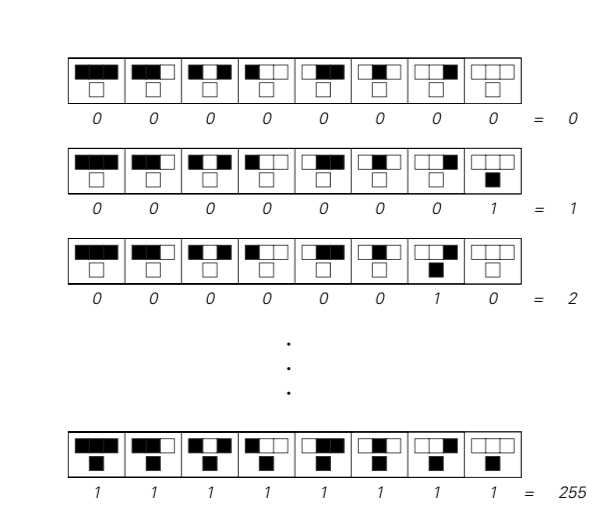
\includegraphics[height=0.6\textheight]{slike/PossibleRules.jpeg}
        \end{column}
    \end{columns}
\end{frame}

\begin{frame}{}
  \begin{block}{}
	In 1982, Conway and others showed Life can simulate:
	\begin{itemize}
	\item memory cells
	\item wires
	\item a clock
	\item logic gates
	\end{itemize}
  \end{block}
  \begin{block}{}
	In 2000, Rendell implemented a Turing Machine in Life, and extended it to a
	universal Turing Machine in 2010.
  \end{block}
\end{frame}

\begin{frame}{Basic concepts for the construction}
  \begin{columns}
	\begin{column}{0.5\textwidth}
	  \begin{itemize}
	  \item gliders transmit information
	  \item a glider's presence = 1, absence = 0
	  \item glider guns repeatedly create gliders
	  \item collide gliders to compute with data
	  \end{itemize}
	\end{column}
	\begin{column}{0.49\textwidth}
	  \animategraphics[loop,autoplay,width=\textwidth]{10}{glider-gun-}{0}{29}
	\end{column}
  \end{columns}
\end{frame}

\begin{frame}{Memory cells}
  \begin{columns}
	\begin{column}{0.5\textwidth}
	  \begin{itemize}
	  \item information stored in circling gliders
	  \item gliders duplicated when we wish to read stored value
	  \item read is triggered by gliders hitting pentadecathlon at top right
	  \end{itemize}
	\end{column}
	\begin{column}{0.5\textwidth}
	  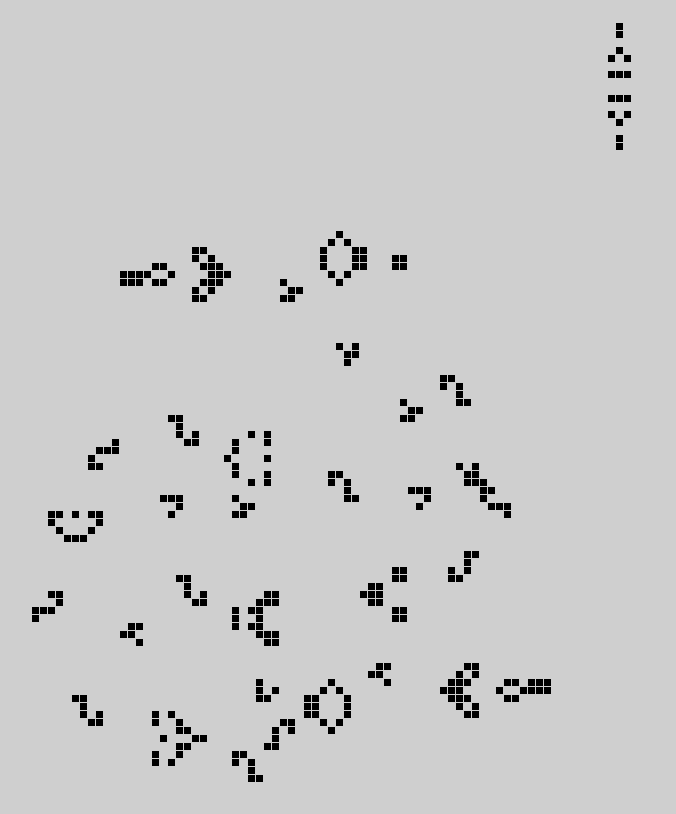
\includegraphics[width=\textwidth]{memory-cell}
	\end{column}
  \end{columns}
\end{frame}

\begin{frame}{The transition function}
  \begin{columns}
	\begin{column}{0.5\textwidth}
	  \begin{itemize}
	  \item grid of memory cells
	  \item rows indexed by state, columns indexed by symbol
	  \item each memory cell contains enough information for a transition: new
		state, new symbol and motion
	  \end{itemize}
	\end{column}
	\begin{column}{0.5\textwidth}
	  \centering
	  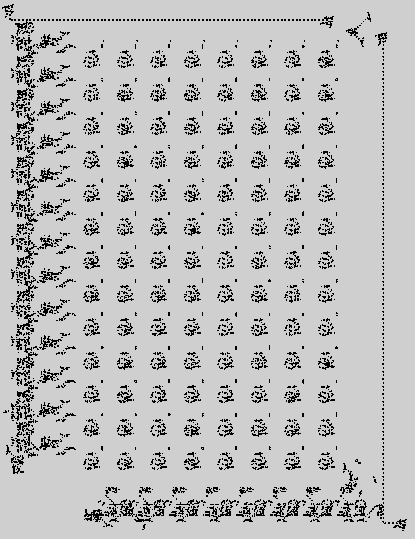
\includegraphics[width=0.92\textwidth]{transition-function}
	\end{column}
  \end{columns}
\end{frame}

\begin{frame}{The tape}
  \begin{columns}
	\begin{column}{0.5\textwidth}
	  \begin{itemize}
	  \item two stacks instead of a tape
	  \item tape motion is performed by a pop and push operation
	  \item no memory cell for symbol at current head position
	  \end{itemize}
	\end{column}
	\begin{column}{0.5\textwidth}
	  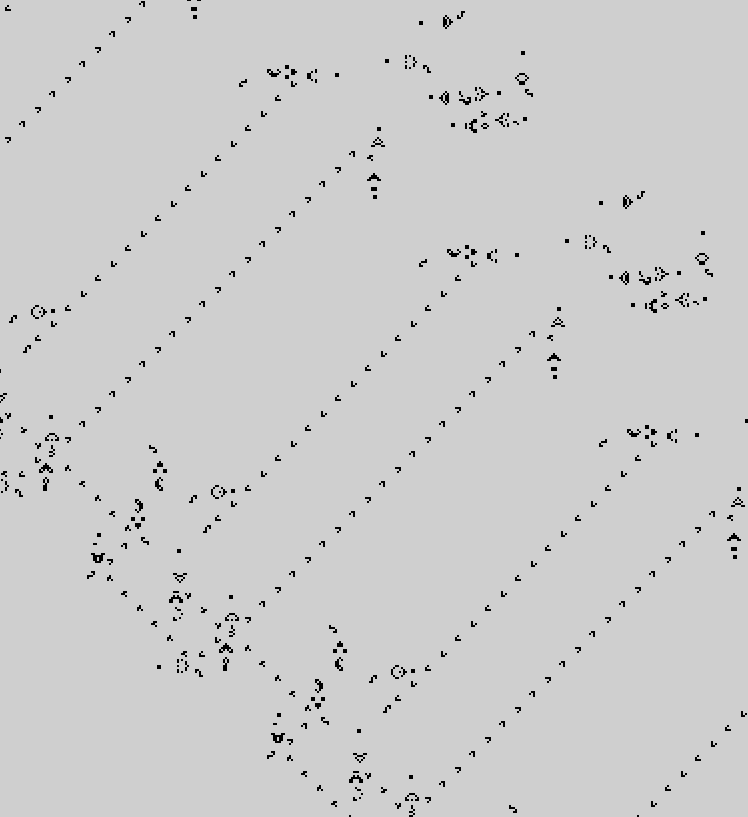
\includegraphics[width=\textwidth]{tape}
	\end{column}
  \end{columns}
\end{frame}

\begin{frame}{The full Turing machine}
  \centering
  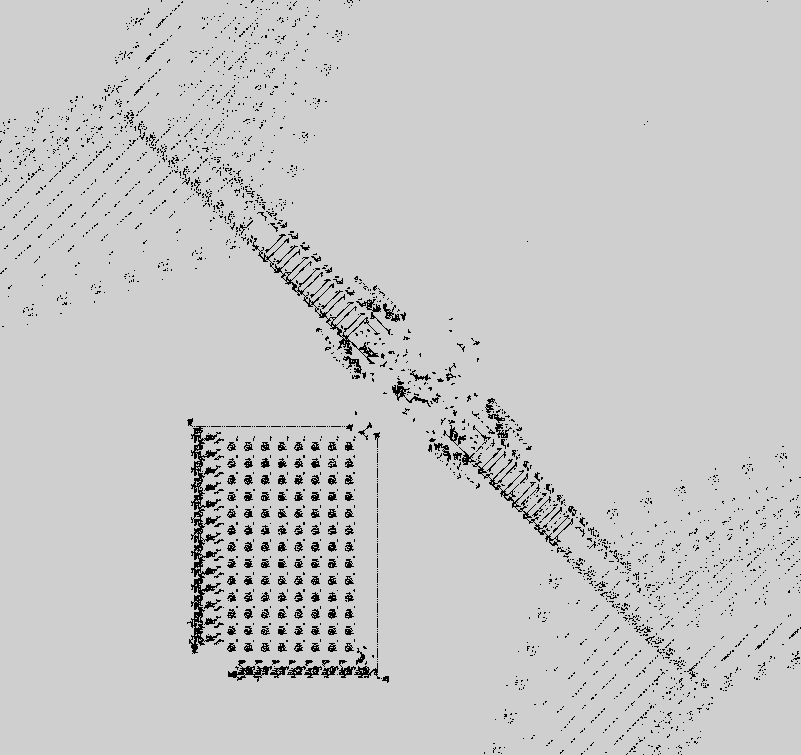
\includegraphics[width=0.6\textwidth]{full}
\end{frame}

\end{document}
